\documentclass[12pt]{article}

\usepackage{amsmath}
\usepackage{amssymb}
\usepackage{graphicx}

\counterwithin*{equation}{section}
\counterwithin*{equation}{subsection}

\graphicspath{ {./images/} } 

\begin{document}
\section{Curves in Polar Coordinates}
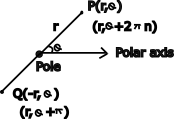
\includegraphics{polarcoordinates}\\%
Polar coordinates are constructed by the distance from the origin $a$ (radius) and the angle $\theta$.\\%
Previously, we used \underline{Rectangular Coordinates}\\%
\underline{Conversions}


\end{document}

